\section{Постановки задачи глобальной оптимизации, обзор существующих методов решения}

\subsection{Задача глобальной оптимизации с функциональными ограничениями-неравенствами}
В рамках данной работы будем рассматривать следующую постановку задачи глобальной
оптимизации: найти глобальный минимум \(N\)-мерной функции \(\varphi(y)\) в гиперинтервале
\(D=\{y\in \mathbf{R}^N:a_i\leqslant x_i\leqslant{b_i}, 1\leqslant{i}\leqslant{N}\}\).
Для построения оценки глобального минимума по конечному количеству вычислений
значения функции требуется, чтобы скорость изменения \(\varphi(y)\) в \(D\) была ограничена.
В качестве такого ограничения как правило принимается условие Липшица.
\begin{equation}
\label{eq:task}
\varphi(y^*)=\min\{\varphi(y):y\in D\}
\end{equation}

\begin{equation}
\label{eq:lip}
|\varphi(y_1)-\varphi(y_2)|\leqslant L\Vert y_1-y_2\Vert,y_1,y_2\in D,0<L<\infty
\end{equation}

Существуют различные методы, решающие рассмотренную многомерную задачу напрямую \cite{SergeyevKvasov2017, Jones2009},
а также эффективные методы решения одномерных задач \cite{Norkin1992, Strongin2000}. В данной работе рассматривается одномерный метод,
который применяется совместно со схемой редукции размерности.
Классической схемой редукции размерности исходной задачи для алгоритмов глобальной оптимизации является
использование разверток --- кривых, заполняющих пространство \cite{Sergeyev2013}.
\begin{equation}
\label{cube}
\lbrace y\in \mathbf{R}^N:-2^{-1}\leqslant y_i\leqslant 2^{-1},1\leqslant i\leqslant N\rbrace=\{y(x):0\leqslant x\leqslant 1\}
\end{equation}

Отображение вида (\ref{cube}) позволяет свести задачу в многомерном пространстве к решению
одномерной ценой ухудшения ее свойств. В частности, одномерная функция \(\varphi(y(x))\)
является не Липшицевой, а Гёльдеровой:
\begin{displaymath}
\label{holder}
|\varphi(y(x_1))-\varphi(y(x_2))|\leqslant H{|x_1-x_2|}^{\frac{1}{N}},x_1,x_2\in[0;1],
\end{displaymath}
где константа Гельдера \(H\) связана с константой Липшица \(L\) соотношением
\begin{equation}
  \label{eq:conv_cond}
 %H=4Ld\sqrt{N},d=\max\{b_i-a_i:1\leqslant i\leqslant N\}.
 H\leqslant 2L\sqrt{N+3}
\end{equation}

Область допустимых аргументов целевой функции также может быть задана с помощью функциональных ограничений, что
значительно усложняет задачу.
Постановка задачи глобальной оптимизации в этом случае будет иметь следующий вид:
\begin{equation}
  \label{eq:constrained_problem}
  \varphi(y^*)=\min\{\varphi(y):y\in D,\: g_j(y)\leqslant 0, 1\leqslant j\leqslant m\}
\end{equation}
Обозначим \(g_{m+1}(y)=\varphi(y)\). Далее будем предполагать, что все функции \(g_k(y),1\leqslant k \leqslant m+1\)
удовлетворяют условию Липшица на гиперинтервале \(D\).

\subsection{Совместное решение серии задач глобальной оптимизации}

Также будем интересоваться совместным решением серии из \(q\) задач вида (\ref{eq:constrained_problem}):
\begin{equation}
  \label{eq:many_problems}
  \min\left\{\varphi_1(y), y\in D_1 \right\}, \min\left\{\varphi_2(y), y\in D_2\right\},..., \min\left\{\varphi_q(y), y\in D_q\right\}.
\end{equation}
Требуется получить приближённое решение во всех задачах их серии, потратив на это как можно меньшее количество испытаний.
При решении серии задач (\ref{eq:many_problems}) возникает проблема оптимального распределения ресурсов метода между ними.
Будем считать, что метод оптимально распоряжается ресурсами, если при его остановке на некоторой итерации
решение всех задач получено с одинаковой точностью. Такого свойства можно добиться, потребовав
от метода равномерной сходимости на всём множестве задач:
\begin{equation}
  \label{eq:uni_conv}
  \exists \varepsilon > 0: \forall s>1, \forall i,j\in\{1,\dots,q\}\;
    \frac{\Vert \tilde{y_i}(s)^* - y_i*\Vert_\infty}{\Vert \tilde{y_j}(s)^* - y^*_j\Vert_	\infty} \leqslant \varepsilon,
\end{equation}
где \(s\) это количество итераций метода оптимизации, \(\tilde{y_i}(s)^*\) это приближение к решению, полученное методом в задаче \(i\)
из множества (\ref{eq:many_problems}) на итерации \(s\).

\subsection{Различные подходы к решению задач глобальной оптимизации}

Одним из возможных способов классификации алгоритмов глобальной оптимизации является разделение их
на детерминированные и стохастические. Стохастические алгоритмы в том или ином виде используют в своей работе
случайные переменные и поэтому результат их работы, вообще говоря, меняется от запуска к запуску. Детерминированные методы
работают по заранее установленным решающим правилам, результат их работы определяется только задачей и,
возможно, некоторыми настраиваемыми параметрами.

\subsubsection{Стохастические методы}

В последнее время стали популярны различные стохастические алгоритмы глобально оптимизации,
прежде всего эволюционные \cite{Storn1997, SCHLUTER2009, KennedyEberhart1995}.
Они имеют довольно простую структуру, позволяют решать задачи большой размерности,
однако обеспечивают глобальную сходимость только в вероятностном смысле. Общим недостатком
стохастических методов является их зависимость от случайных переменных и, в силу характера сходимости,
начальной точки, с которой начинается оптимизация (она может также генерироваться случайно).
Примерами неэволюционных стратегий стохастической оптимизации являются случайный поиск \cite{rastrigin1963},
метод имитации отжига \cite{XIANG1997216} и муравьиный алгоритм \cite{ZhangACO2008}. Стоит отметить, что
стохастические методы поиска не требуют дифференцируемости или даже непрерывности от целевой функции задачи оптимизации,
могут работать с зашумлёнными функциями.

\subsubsection{Детерминированные методы}

Стохастические методы обладают одним концептуальным недостатком -- нельзя гарантировать их сходимость при
каждом конкретном запуске процесса оптимизации. Для детерминированных методов есть возможность построить теорию сходимости,
наложив ограничения на скорость изменения целевой функции в задаче (\ref{eq:task}). Если этого не сделать, то
по любому конечному количеству значений целевой функции невозможно построить её модель с гарантированной нижней оценкой.
Известным и широко представленным классом детерминированных методов являются методы липшицевой оптимизации, предполагающие
Липшиц-непрерывность целевой функции в задаче оптимизации. В одномерном случае к таким методам можно отнести семейство
характеристических методов \cite{gorodetsky2007}, в которое входит, например, метод Пиявского \cite{pijavsky1972} и AGS \cite{strongin1978}.
Для их применение в случае многомерных задач используются схемы редукции размерности \cite{strongin1978}.
Методы диагональных \cite{Sergeyev2015} или симплексных \cite{Zilinskas2014} разбиений не требуют использования
таких схем, однако более сложны в реализации, т.к. требуется эффективно хранить и модифицировать множество многомерных гиперинтервалов
или симплексов.

\paragraph{Индексный алгоритм глобального поиска}
В качестве примера детерминированного характеристического метода приведём индексный алгоритм глобального поиска \cite{Strongin2000}.

Принимая во внимание схему редукции размерности (\ref{cube}), будем при описании метода считать, что
требуется найти глобальный минимум функции \(\varphi(x), x\in[0;1]\),
удовлетворяющей условию Гёльдера, при ограничениях \(g_j(x)\), также
удовлетворяющих этому условию на интервале \([0;1]\).

Рассматриваемый индексный алгоритм глобального поиска (IAGS) для решения
одномерной задачи (\ref{eq:constrained_problem}) предполагает построение последовательности
точек \(x_k\), в которых вычисляются значения минимизируемой функции или ограничений \(z_k = g_s(x_k)\).
Для учета последних используется индексная схема \cite{Strongin2000}. Пусть \(Q_0=[0;1]\). Ограничение, имеющее номер
 \(j\), выполняется во всех точках области
\begin{displaymath}
  Q_j=\left\{x\in [0;1]:g_j(x)\leq 0\right\},
\end{displaymath}
которая называется допустимой для этого ограничения. При этом допустимая область \(D\)
исходной задачи определяется равенством: \(D=\cap _{j=0}^{m}Q_{j}\).
Испытание в точке \(x\in [0;1]\) состоит в последовательном вычислении значений
величин \(g_{1}(x),...,g_{\nu }(x)\), где значение индекса \(\nu\) определяется условиями:
\(x\in Q_{j},0\leqslant j<\nu ,x\notin Q_{\nu }\). Выявление первого нарушенного ограничения
прерывает испытание в точке \(x\). В случае, когда точка \(x\)  допустима, т. е.
\(x\in D\) испытание включает в себя вычисление всех функций задачи. При этом значение
индекса принимается равным величине \(\nu =m+1\). Пара \(\nu =\nu (x),z=g_{\nu }(x)\),
где индекс \(\nu\) лежит в границах \(1\leqslant \nu \leqslant m+1\), называется результатом
испытания в точке \(x\).

Такой подход к проведению испытаний позволяет свести исходную задачу с функциональными
ограничениями к безусловной задаче минимизации разрывной функции:

\begin{displaymath}
  \begin{array}{lr}
    \psi (x^{*})=\min_{x\in [0;1]}\psi (x), \\
    \psi (x)={\begin{cases}g_{\nu }(x)/H_{\nu }&\nu <M\\(g_{M}(x)-g_{M}^{*})/H_{M}&\nu =M\end{cases}}
  \end{array}
\end{displaymath}

Здесь \(M=\max_{}^{}\left\{\nu (x):x\in [0;1]\right\}\), а \(g_{M}^{*}=\min _{}^{}\left\{g_{M}(x):x\in \cap _{i=0}^{M-1}Q_{i}\right\}\).
В силу определения числа \(M\), задача отыскания \(g_{M}^{*}\)
всегда имеет решение, а если \(M=m+1\), то \(g_{M}^{*}=\varphi(x^{*})\).
Дуги функции \(\psi (x)\) гельдеровы на множествах \(\cap _{i=0}^{j}Q_{i},0\leq j\leq M-1\)
с константой 1, а сама \(\psi (x)\) может иметь разрывы первого рода на границах этих множеств.
Несмотря на то, что значения констант Гёльдера \(H_k\) и величина \(g_{M}^{*}\) заранее неизвестны,
они могут быть оценены в процессе решения задачи.

Множество троек \(\{(x_k,\nu_k,z_k)\}, 1\leqslant k\leqslant n\) составляет поисковую информацию,
накопленную методом после проведения \(n\) шагов.

На первой итерации метода испытание проводится в произвольной внутренней точке \(x_1\)
интервала \([0;1]\). Индексы точек 0 и 1 считаются нулевыми, значения \(z\) в
них не определены. Пусть выполнено \(k\geqslant 1\) итераций метода,
в процессе которых были проведены испытания в \(k\) точках \(x_i, 1\leqslant i\leqslant k\).
Тогда точка \(x^{k+1}\) поисковых испытаний следующей \((k+1)\)-ой
итерации определяются в соответствии с правилами:

Шаг 1. Перенумеровать точки множества \(X_k=\{x^1,\dotsc,x^k\}\cup\{0\}\cup\{1\}\),
которое включает в себя граничные точки интервала \([0;1]\), а также точки предшествующих
испытаний, нижними индексами в порядке увеличения значений координаты, т.е.
\begin{equation}
  \label{eq:points}
0=x_0<x_1<\dotsc<x_{k+1}=1
\end{equation}
и сопоставить им значения \(z_{i}=g_{\nu }(x_{i}),\nu =\nu (x_{i}),i={\overline {1,k}}\).

Шаг 2. Для каждого целого числа \(\nu ,1\leqslant \nu \leqslant m+1\) определить соответствующее
ему множество \(I_{\nu }\) нижних индексов точек, в которых вычислялись значения
функций \(g_{\nu }(x)\):
\begin{displaymath}
  I_{\nu }=\{i:\nu (x_{i})=\nu ,1\leqslant i\leqslant k\},1\leq \nu \leqslant m+1,
\end{displaymath}
определить максимальное значение индекса \(M=\max\{\nu (x_{i}),1\leq i\leq k\}\).

Шаг 3. Вычислить текущие оценки для неизвестных констант Гёльдера:
\begin{equation}
  \label{eq:step2}
  \mu _{\nu }=\max\{\frac{|g_{\nu }(x_{i})-g_{\nu }(x_{j})|}{(x_{i}-x_{j})^{\frac{1}{N}}}:i,j\in I_{\nu },i>j\}.
\end{equation}
Если множество \(I_{\nu }\) содержит менее двух элементов или если значение \(\mu _{\nu }\)
оказывается равным нулю, то принять \(\mu _{\nu }=1\).

Шаг 4. Для всех непустых множеств \(I_{\nu },\nu ={\overline {1,M}}\) вычислить оценки
\begin{equation}
  \label{eq:step_4}
  z_{\nu }^{*}={\begin{cases}\min\{g_{\nu }(x_{i}):x_{i}\in I_{\nu }\}&\nu =M\\-\varepsilon _{\nu }&\nu <M\end{cases}},
\end{equation}
где вектор с неотрицательными координатами \(\varepsilon _{R}=(\varepsilon _{1},..,\varepsilon _{m})\) называется вектором резервов.

Шаг 5. Для каждого интервала \((x_{i-1};x_{i}),1\leqslant i\leqslant k\) вычислить характеристику
\begin{equation}
  \label{eq:step3_1}
  R(i)={\begin{cases}\Delta _{i}+{\frac {(z_{i}-z_{i-1})^{2}}{(r_{\nu }\mu _{\nu })^{2}\Delta _{i}}}-2{\frac {z_{i}+z_{i-1}-2z_{\nu }^{*}}{r_{\nu }\mu _{\nu }}}&\nu =\nu (x_{i})=\nu (x_{i-1})\\2\Delta _{i}-4{\frac {z_{i-1}-z_{\nu }^{*}}{r_{\nu }\mu _{\nu }}}&\nu =\nu (x_{i-1})>\nu (x_{i})\\2\Delta _{i}-4{\frac {z_{i}-z_{\nu }^{*}}{r_{\nu }\mu _{\nu }}}&\nu =\nu (x_{i})>\nu (x_{i-1})\end{cases}}
\end{equation}
где \(\Delta _{i}=(x_{i}-x_{i-1})^{\frac{1}{N}}\). Величины \(r_{\nu }>1,\nu ={\overline {1,m}}\)
являются параметрами алгоритма. От них зависят произведения \(r_{\nu }\mu _{\nu }\),
используемые при вычислении характеристик в качестве оценок неизвестных констант Гёльдера.

Шаг 6. Выбрать наибольшую характеристику:
\begin{equation}
\label{step4}
t=\argmax_{1\leqslant i \leqslant k+1}R(i)
\end{equation}

Шаг 7. Провести очередное испытание в середине интервала \((x_{t-1};x_{t})\),
если индексы его концевых точек не совпадают: \(x^{k+1}={\frac {1}{2}}(x_{t}+x_{t-1})\).
В противном случае провести испытание в точке
\begin{displaymath}
  x^{k+1}={\frac {1}{2}}(x_{t}+x_{t-1})-\operatorname {sgn}(z_{t}-z_{t-1}){\frac {|z_{t}-z_{t-1}|^{n}}{2r_{\nu }\mu _{\nu }^{n}}},\nu =\nu (x_{t})=\nu (x_{t-1}),
\end{displaymath}
а затем увеличить \(k\) на 1.

Алгоритм прекращает работу, если выполняется условие \(\Delta_{t}\leqslant \varepsilon\),
где \(\varepsilon>0\) есть заданная точность. В качестве оценки глобально-оптимального решения выбираются значения
\begin{equation}
\varphi_k^*=\min_{1\leqslant i \leqslant k}\varphi(x_i), x_k^*=\argmin_{1\leqslant i \leqslant k}\varphi(x_i)
\end{equation}

Теорема о сходимости для этого метода подробно рассмотрена в \cite{Strongin2000}, а также будет рассматриваться в главе \ref{sec:conv_method}.
Здесь отметим лишь, что путём увеличения \(r\) и при \(\varepsilon=0\) можно гарантированно добиться сходимости,
если все функции задачи (\ref{eq:constrained_problem}) удовлетворяют условию Липшица на гиперкубе из (\ref{eq:task}).

\section{Подходы к сравнению алгоритмов глобальной оптимизации}
\label{sec:comp_tools}
Основным подходом к сравнению между собой методов оптимизации является запуск этих методов на наборах тестовых задач
и последующее сравнение собранных в процессе запуска метрик, характеризующие различные аспекты работы алгоритмов.
Исключая некоторые специальные случаи, когда требуется определить метод, лучше других себя ведущий на небольшом наборе специфичных задач
или вообще на одной задаче с параметром. Существуют два способа построить тестовый набор задач: собрать небольшое множество
известных из литературы тестовых задач \cite{kampfComparison2010} или использовать рандомизированные генераторы задач, позволяющие генерировать потенциально
любое количество задач \cite{Gaviano2003, grishaginClass}. В \cite{Beiranvand2017} подробно рассмотрены недостатки и достоинства каждого из
подходов. Известных тестовых задач мало, поэтому используя только их не всегда можно достаточно полно выявить особенности работы различных методов.
В то же время генераторы задач позволяют создать любое их количество, однако полученные задачи могут обладать скрытой общей структурой, благоприятной для
некоторых из тестируемых методов, либо обладать малой вариативностью. Поскольку в рамках работы рассматриваются алгоритмы
для решения существенно многоэкстремальных задач, будем производить все сравнения на задачах, полученных с помощью нескольких генераторов
достаточно таких задач. Это сгладит проблему потенциально низкой вариативности задач, полученных одним генератором. Также в одном специальном
случае рассмотрим решение одной известной задачи из литературы \cite{BinhKorn1999}.

В рамках данной работы будем использовать два механизма генерации тестовых задач \cite{grishaginClass, Gaviano2003} \footnote{Программные реализации
генераторов доступны в исходных кодах по адресу \url{https://github.com/sovrasov/global-optimization-test-problems}}. Тестовые задачи, получаемые
данными механизмами, имеют абсолютно разную природу (см. линии уровня на Рис. \ref{fig:isolines_unconstrained}),
что увеличивает достоверность результатов сравнения алгоритмов оптимизации.

\begin{figure}[ht]
  \centering
  \subfloat[Пример линий уровня функции, порождённой \(F_{GR}\)]{
  {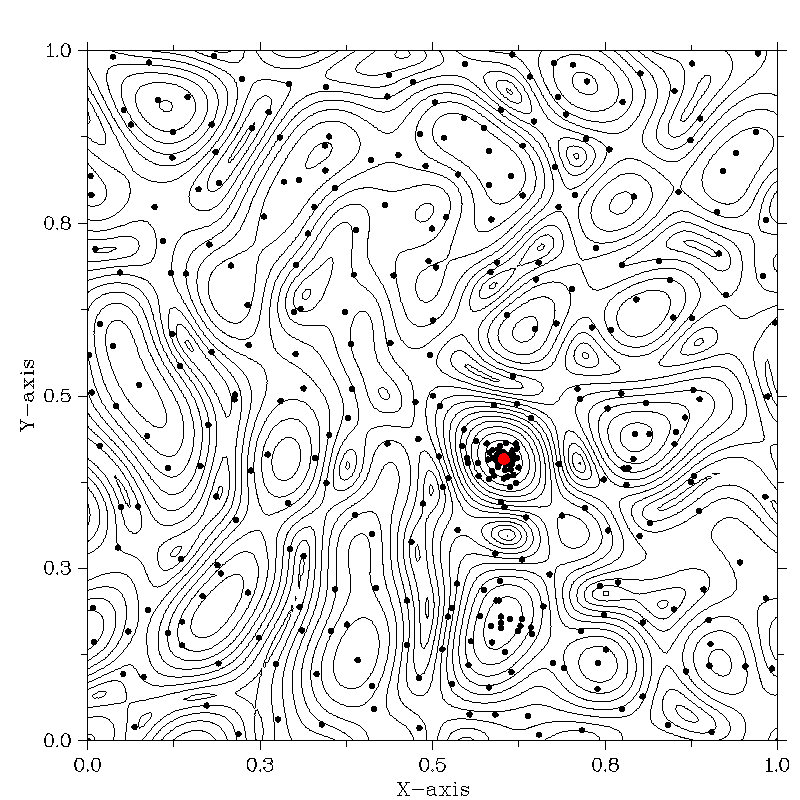
\includegraphics[width=.5\textwidth]{gs_loc.png}}}
  \subfloat[Пример линий уровня функции, порождённой GKLS]{
  {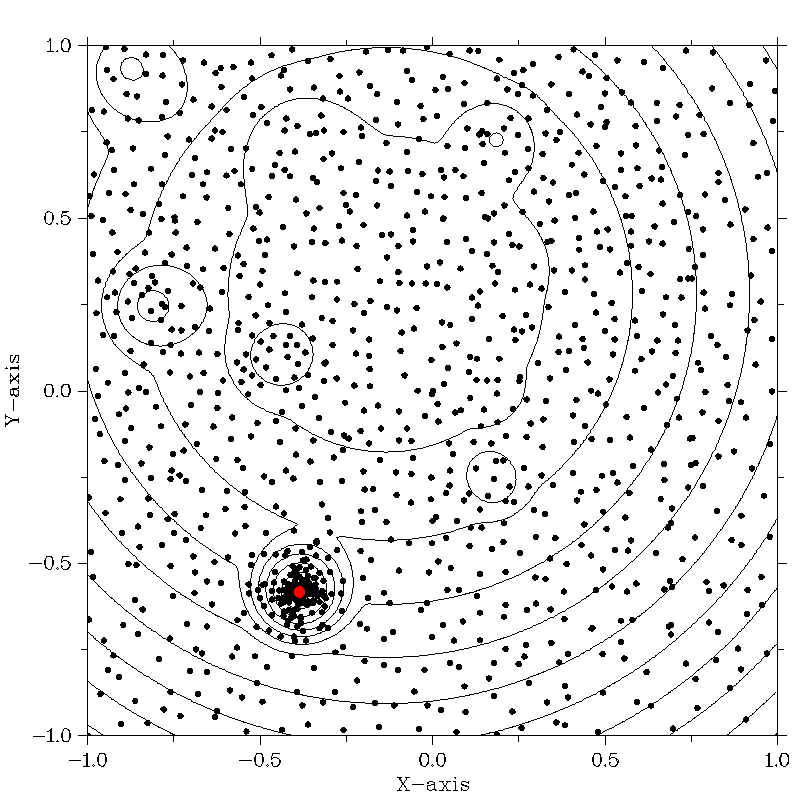
\includegraphics[width=.5\textwidth]{gkls_loc.png}}}
  \caption{Линии уровня и точки испытаний ИАГП в двух синтетических задачах без ограничений}
  \label{fig:isolines_unconstrained}
\end{figure}

Обозначим набор двумерных задач, полученный с помощью генератора \cite{grishaginClass}
как \(F_{GR}\). Генератор \(F_{GR}\) не позволяет контролировать размерность и сложность задач, а также количество локальных экстремумов.
Каждая тестовая задача определяется формулой:
\begin{displaymath}
  \varphi(y)=\sqrt{\left(\sum_{i=1}^7\sum_{j-1}^7 A_{ij}g_{ij}(y)+ B_{ij}h_{ij}(y)\right)^2+\left(\sum_{i=1}^7\sum_{j-1}^7 C_{ij}g_{ij}(y) - D_{ij}h_{ij}(y)\right)^2}
\end{displaymath}
где
\begin{displaymath}
  \begin{array}{cr}
    y\in[0;1]^2, \\
    g_{ij}=\sin(i\pi y_1)\sin(j\pi y_2), \\
    h_{ij}=\cos(i\pi y_1)\cos(j\pi y_2),
  \end{array}
\end{displaymath}
где коэффициенты \(A_{ij},B_{ij}, C_{ij}, D_{ij}\) генерируются случайно с равномерным в
интервале \([-1;1]\) распределением.
Получаемые функции являются существенно многоэкстремальными. В данной работе будем использовать 100 функций, сгенерированных с помощью \(F_{GR}\).

Геренатор GKLS \cite{Gaviano2003} позволяет получать тестовые задачи заданной размерности с заданным количеством локальных
экстремумов. Также этот генератор позволяет варьировать сложность задачи, изменяя размер области притяжения
глобального минимума. Это достигается за счёт модификации параболоида \(g(x)=\Vert x-T\Vert + t\) в
шаровых окрестностях некоторых случайно сгенерированных точек \(M_i, i=\overline{1,m}\). В точках
\(M_i\) располагаются локальные минимумы со значениями, превосходящими значение \(g(T)=t\).
В \cite{SergeyevKvasov2006} приводятся параметры генератора для получения
наборов по 100 задач двух уровней сложности (Simple and Hard) размерностей 2, 3, 4 и 5.
Как и авторы генератора GKLS, будем использовать эти параметры и таким образом получим 800 тестовых задач.

Перечисленные выше генераторы порождают задачи без нелинейных ограничений, поэтому в дополнение к ним будем использовать
систему GCGen \footnote{Исходный код системы доступен по ссылке \url{https://github.com/UNN-ITMM-Software/GCGen}}
\cite{GergelBarkalov2019}, которая позволяет генерировать задачи с ограничениями на основе произвольных нелинейных
функций. При использовании этой системы совместно с генераторами, таким как GKLS, порождённые ими функции выступают как
в роли целевой функции, так и в роли ограничений.

С помощью GCGen были сгенерированы следующие наборы задач с ограничениями:
\begin{itemize}
  \item 100 двумерных задач на основе GKLS Simple 2d с двумя ограничениями;
  \item 100 трёхмерных задач на основе GKLS Simple 3d с двумя ограничениями;
  \item 20 четырёхмерных задач на основе GKLS Simple 4d с двумя ограничениями;
  \item смешанный набор, состоящий из 50 задач на основе GKLS Simple 2d и 50 задач на основе \(F_{GR}\).
  Каждая задача имеет два функциональных ограничения. Этот набор позволяет проверить наличие у метода оптимизации
  свойства равномерной сходимости при решении множества задач в постановке (\ref{eq:many_problems}).
\end{itemize}

Генератор GKLS \cite{Gaviano2003} позволяет получать функции заданной размерности и с заданным количеством экстремумов.
В сочетании с GCGen были порождены два множества по 100 задач размерности 2 и 3. Каждая из задач имеет два ограничения.
Также с целью демонстрации того, что свойства метода сохраняются при существенно разных свойствах задач
был сгенерирован смешанный класс, состоящий из 50 задач с двухмерными функциями GKLS и 50 задач с функциями \(F_{GR}\).
На рис. \ref{fig:isolines} представлены примеры линий уровня рассматриваемых задач. Допустимая область закрашена.

\begin{figure}[ht]
    \centering
    \subfloat[Решение внутри допустимой области]{
    {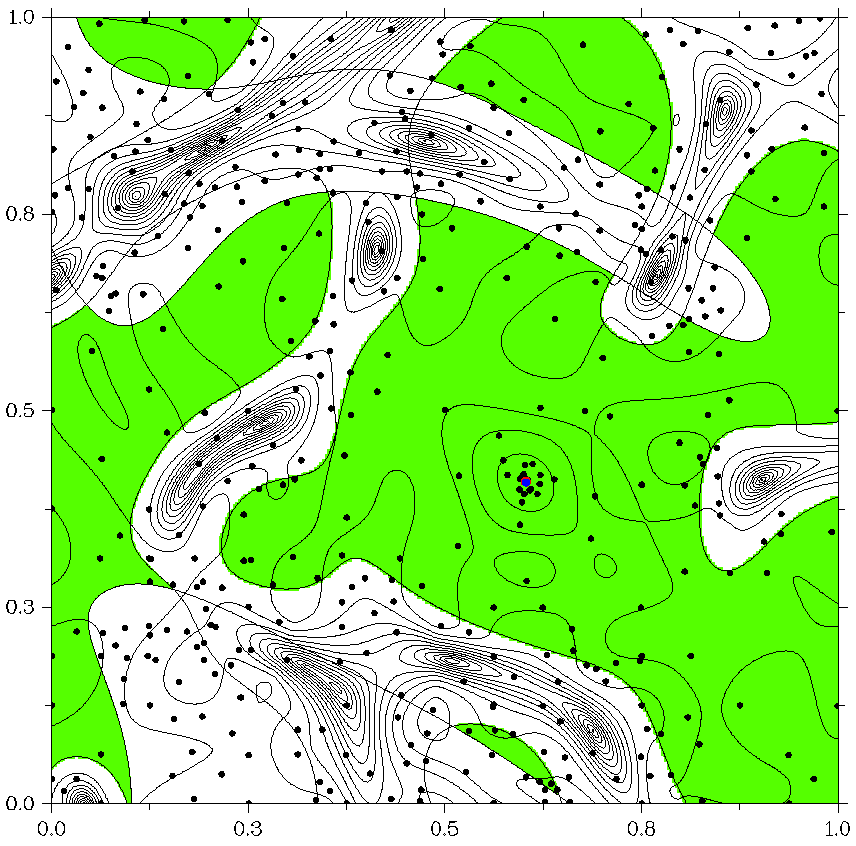
\includegraphics[width=.5\textwidth]{images/2.png}}}
    \subfloat[Решение на границе допустимой области]{
    {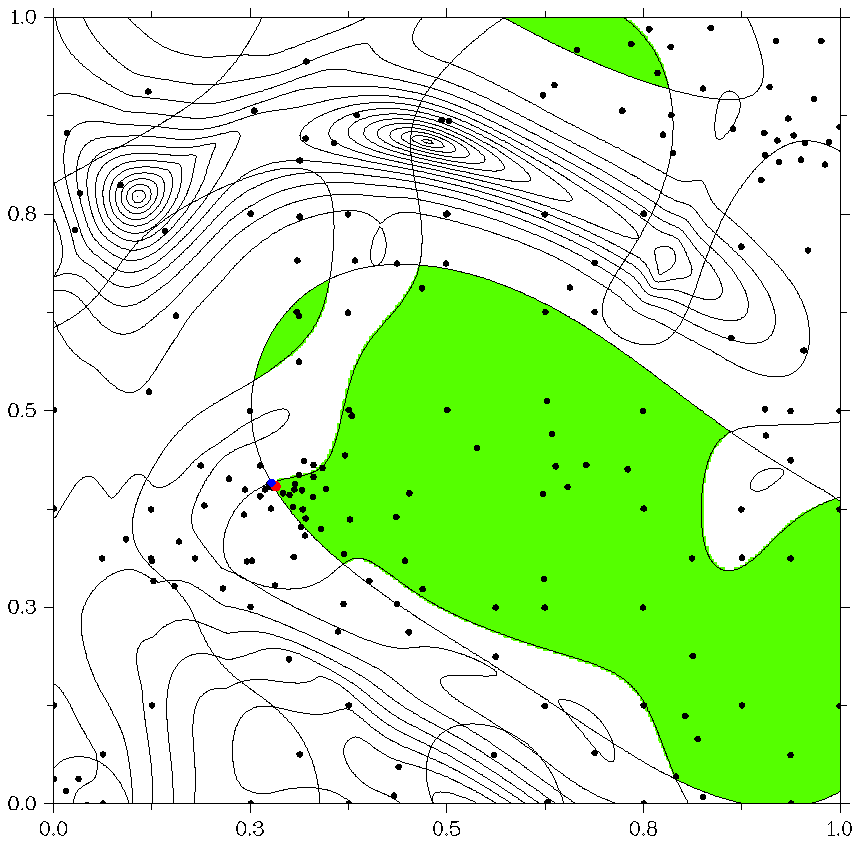
\includegraphics[width=.5\textwidth]{images/4.png}}}
    \caption{Линии уровня и точки испытаний ИАГП в двух синтетических задачах}
    \label{fig:isolines}
\end{figure}


Будем считать, что тестовая задача решена, если метод выполняет испытание
\(y^k\) в \(\delta\)-окрестности глобального минимума \(y^*\), т.е. $\left\|y^k-y^*\right\|_{inf}\leq \delta
= \alpha\left\|b-a\right\|_{inf}$, где \(a\) и \(b\) это правая и левая границы гиперкуба из (\ref{eq:task}),
а $\alpha$ это относительная точность. Если указанное соотношение не выполнено до исчерпания лимита на
испытания, то задача считается нерешённой. Лимит на количество испытаний и $\alpha$ заданы для каждого класса задач в отдельности
в соответствии с размерностью задач и их сложностью (см. Таблицу \ref{tab:limits}).

\begin{table}
\begin{center}
\caption{Лимит на количество испытаний и относительная точность в критерии остановки для различных классов задач}
  \begin{tabular}{|l|{c}|{c}|}
    \hline
  Problems class & Trials limit & $\alpha$\\
  \hline
  \(F_{GR}\) & 5000 & 0.01 \\
  \hline
  GKLS 2d Simple & 8000 & 0.01 \\
  \hline
  GKLS 2d Hard & 9000 & 0.01 \\
  \hline
  GKLS 3d Simple & 15000 & 0.01 \\
  \hline
  GKLS 3d Hard & 25000 & 0.01 \\
  \hline
  GKLS 4d Simple & 150000 & $\sqrt[4]{10^{-6}}$ \\
  \hline
  GKLS 4d Hard & 250000 & $\sqrt[4]{10^{-6}}$ \\
  \hline
  GKLS 5d Simple & 350000 & $\sqrt[5]{10^{-7}}$ \\
  \hline
  GKLS 5d Hard & 600000 & $\sqrt[5]{10^{-7}}$ \\
  \hline
  \end{tabular}
  \label{tab:limits}
\end{center}
\end{table}

Будем рассматривать среднее количество испытаний, затраченное на решение одной задачи, и количество
решенных задач как характеристики эффективности метода оптимизации на заданном классе задач.
Чем меньше среднее количество испытаний на задачу, тем быстрее метод сходится к решению, а значит и
меньше обращается к потенциально трудоёмкой процедуре вычисления ограничений и целевой функции задачи.
Количество решённых задач характеризует надёжность метода. Чтобы сделать рассматриваемые характеристики независимыми друг от друга,
будем вычислять среднее количество испытаний, принимая во внимание только решённые задачи.

Среднее число испытаний на задачу в некоторых случаях не позволяет получить полной картины о
поведении численного метода оптимизации на рассматриваемом множестве задач. Например, если метод
тратит много ресурсов на решение небольшого подмножества задач из выборки, то это невозможно понять,
глядя только на среднее число испытаний. Как дополнительный критерий сравнения методов будем
использовать операционную характеристику \cite{grishaginClass}. Операционная характеристика
представляет из себя кривую на плоскости \((K, P)\), где \(K\) это среднее количество испытаний,
произведённое методом до выполнения критерия остановки, а \(P\) -- доля задач из выборки, решённых не более чем за \(K\)
испытаний. Если при заданном \(K\) операционная характеристика одного метода лежит выше, чем
операционная характеристика другого, то это означает, что при фиксированных затратах на поиск,
первый метод с большей вероятностью найдёт решение. При заданном \(P\) если характеристика одного метода лежит левее,
чем характеристика другого, то при одинаковой надёжности, первый метод в среднем потратит меньше испытаний на поиск, чем второй.
